\phantomsection
\section*{Chapter 6}
\addcontentsline{toc}{section}{Chapter 6}

\subsection*{6.3}

\begin{figure}[H]
  \centering
  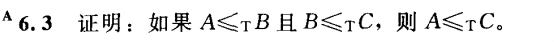
\includegraphics[width=\textwidth]{chapters/imgs/hw_6_3.png}
  \caption{}
  \label{fig:hw_6_3}
\end{figure}

\begin{answerred}
证明。假设
\[
    A \le_T B
    \qquad\text{且}\qquad
    B \le_T C.
\]
由定义，存在一台带预言机 $B$ 的图灵机 $M^B$ 判定 $A$，并且存在一台带预言机 $C$ 的图灵机 $N^C$ 判定 $B$。也就是说，对任意字符串 $x$，
\[
    N^C \text{ 接受 } x
    \iff
    x\in B.
\]

\medskip
构造下面这台带预言机 $C$ 的图灵机 $T^C$。

\begin{quote}
$T^C=$ “在输入 $w$ 上：

\begin{enumerate}[label=\arabic*., leftmargin=2.5em]
  \item 模拟 $M^B$ 在输入 $w$ 上的运行。
  \item 每当被模拟的 $M^B$ 向它的 $B$-预言机询问某个字符串 $x$ 是否属于 $B$ 时，执行下面的子过程：
  \begin{enumerate}[label=\arabic*., leftmargin=2.5em]
    \item 在输入 $x$ 上运行 $N^C$。
    \item 如果 $N^C$ 接受，则把这次 $B$-预言机询问回答为 YES；如果 $N^C$ 拒绝，则回答为 NO。
  \end{enumerate}
  \item 按照上一步得到的 oracle 答案继续模拟 $M^B$。
  \item 如果被模拟的 $M^B$ 接受，则接受；如果它拒绝，则拒绝。”
\end{enumerate}
\end{quote}

\medskip
现在证明 $T^C$ 判定 $A$。对每一次 $M^B$ 发出的 $B$-预言机询问
\[
    x\in B\;?
\]
机器 $T^C$ 都用 $N^C(x)$ 来回答。因为 $N^C$ 判定 $B$，所以这个回答与真正的 $B$-预言机给出的回答完全相同。因此，在任意输入 $w$ 上，$T^C$ 对 $M^B(w)$ 的模拟与真正拥有 $B$-预言机时的运行一致。

于是对任意 $w$，
\[
    T^C \text{ 接受 } w
    \iff
    M^B \text{ 接受 } w
    \iff
    w\in A.
\]
此外，$M^B$ 是判定器，所以它在每个输入上只进行有限步计算并最终停机；每次被调用的 $N^C$ 也是判定器，所以每个 oracle 询问的替代计算也会停机。因此 $T^C$ 对每个输入都停机。

\medskip
故 $T^C$ 是一台带预言机 $C$ 的判定器，并且它判定 $A$。所以
\[
    A \le_T C.
\]
这就证明了图灵可归约性的传递性。$\blacksquare$

\begin{answernote}
\paragraph{解释.}
这是预言机版本的“函数复合”。$A\le_T B$ 的意思不是“由 $A$ 判定 $B$”，而是“如果有 $B$ 的答案，就能判定 $A$”。所以在证明传递性时，先用 $M^B$ 把 $A$ 的问题转化成若干个 $B$ 的问题，再用 $N^C$ 把每个 $B$ 的问题转化成 $C$ 的问题，最终得到一个 $T^C$ 来判定 $A$。

\end{answernote}
\end{answerred}
\subsection*{6.4}

\begin{figure}[H]
  \centering
  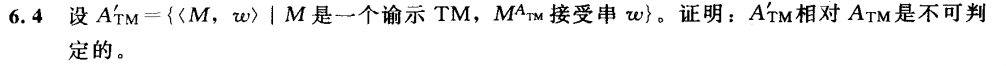
\includegraphics[width=\textwidth]{chapters/imgs/hw_6_4.png}
  \caption{}
  \label{fig:hw_6_4}
\end{figure}

\begin{answerred}
设
\[
    A_{\mathrm{TM}}^{A_{\mathrm{TM}}}
    =
    \{\langle M,w\rangle \mid M \text{ 是预言机图灵机且 } M^{A_{\mathrm{TM}}} \text{ 接受 } w\}.
\]
我们证明：
\[
    A_{\mathrm{TM}}^{A_{\mathrm{TM}}}
\]
相对于预言机
\[
    A_{\mathrm{TM}}
\]
仍然不可判定。

\medskip
反设存在一台带预言机 $A_{\mathrm{TM}}$ 的图灵机 $H^{A_{\mathrm{TM}}}$ 判定
\[
    A_{\mathrm{TM}}^{A_{\mathrm{TM}}}.
\]
也就是说，对任意预言机图灵机 $M$ 和输入 $w$，
\[
    H^{A_{\mathrm{TM}}}(\langle M,w\rangle)
\]
接受当且仅当
\[
    M^{A_{\mathrm{TM}}} \text{ 接受 } w.
\]

\begin{myalgo}{对角化构造的预言机图灵机 $D^{A_{\mathrm{TM}}}$}
\begin{algorithmic}[1]
  \Require 输入 $\langle M\rangle$，其中 $M$ 是预言机图灵机
  \Ensure 与 $M^{A_{\mathrm{TM}}}$ 在输入 $\langle M\rangle$ 上的行为相反
  \State 在输入 $\langle M,\langle M\rangle\rangle$ 上运行 $H^{A_{\mathrm{TM}}}$
  \If{$H^{A_{\mathrm{TM}}}$ 接受}
    \State \textbf{拒绝}
  \Else
    \State \textbf{接受}
  \EndIf
\end{algorithmic}
\end{myalgo}

现在考察 $D^{A_{\mathrm{TM}}}$ 在自身描述上的行为。若
\[
    D^{A_{\mathrm{TM}}} \text{ 接受 } \langle D\rangle,
\]
则按照 $D$ 的定义，
\[
    H^{A_{\mathrm{TM}}}(\langle D,\langle D\rangle\rangle)
\]
必须拒绝。但 $H$ 判定
\[
    A_{\mathrm{TM}}^{A_{\mathrm{TM}}},
\]
因此它拒绝恰意味着
\[
    D^{A_{\mathrm{TM}}}
\]
不接受
\[
    \langle D\rangle,
\]
矛盾。

\medskip
反之，若
\[
    D^{A_{\mathrm{TM}}} \text{ 不接受 } \langle D\rangle,
\]
则 $H^{A_{\mathrm{TM}}}(\langle D,\langle D\rangle\rangle)$ 必须接受，于是按 $D$ 的定义，
\[
    D^{A_{\mathrm{TM}}} \text{ 接受 } \langle D\rangle,
\]
仍然矛盾。

\medskip
故这样的 $H^{A_{\mathrm{TM}}}$ 不存在。于是
\[
    A_{\mathrm{TM}}^{A_{\mathrm{TM}}}
\]
相对于
\[
    A_{\mathrm{TM}}
\]
不可判定。$\blacksquare$

\begin{answernote}
\paragraph{解释.}
这就是普通
\[
    A_{\mathrm{TM}}
\]
不可判定证明的相对化版本。即便机器本身已经拥有
\[
    A_{\mathrm{TM}}
\]
预言机，我们仍然可以对“带这个预言机的机器是否接受”做对角化，所以再强一层的接受问题依然超出这一层预言机的能力。

\end{answernote}
\end{answerred}
\subsection*{6.7}

\begin{figure}[H]
  \centering
  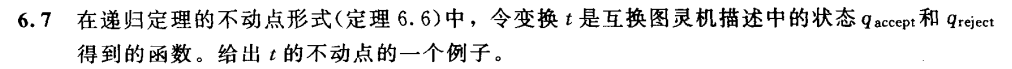
\includegraphics[width=\textwidth]{chapters/imgs/hw_6_7.png}
  \caption{}
  \label{fig:hw_6_7}
\end{figure}

\begin{answerred}
\paragraph{解答.}
令 $t$ 是这样一个可计算变换：对任意图灵机描述
\[
\langle M\rangle,
\]
$t(\langle M\rangle)$ 是把 $M$ 的
\[
q_{\mathrm{accept}}
\quad\text{与}\quad
q_{\mathrm{reject}}
\]
互换后得到的机器描述。

\medskip
在递归定理的不动点形式里，$t$ 的一个不动点是任何满足
\[
L(M)=L(t(\langle M\rangle))
\]
的机器 $M$。一个最简单的例子是：

\begin{center}
\emph{在任意输入上都一直循环、从不进入接受态或拒绝态的图灵机。}
\end{center}

设这台机器为 $M$。那么对任意输入 $w$，
\[
M \text{ 在 } w \text{ 上一直循环},
\]
因此
\[
w\notin L(M).
\]

把
\[
q_{\mathrm{accept}}
\quad\text{和}\quad
q_{\mathrm{reject}}
\]
互换之后，机器的实际运行并没有任何变化，因为这两个状态本来就永远不会被访问到。所以对任意输入 $w$，
\[
t(\langle M\rangle)
\]
也仍然一直循环，从而
\[
w\notin L(t(\langle M\rangle)).
\]

于是
\[
L(M)=\varnothing=L(t(\langle M\rangle)).
\]
故这台“对所有输入都循环”的图灵机就是 $t$ 的一个不动点例子。$\blacksquare$

\begin{answernote}
\paragraph{解释.}
这里的不动点不是说机器描述字面上一模一样，而是说变换前后识别的语言相同。若一台机器从来不进入接受态或拒绝态，那么交换这两个状态根本不会改变它的行为，因此自然就是一个不动点。

\end{answernote}
\end{answerred}
\subsection*{6.10}

\begin{figure}[H]
  \centering
  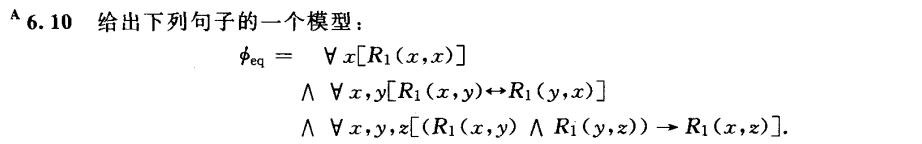
\includegraphics[width=\textwidth]{chapters/imgs/hw_6_10.png}
  \caption{}
  \label{fig:hw_6_10}
\end{figure}

\begin{answerred}
\paragraph{解答.}
一个最简单的模型是
\[
\mathcal M=(\mathbb N,R_1^{\mathcal M}),
\]
其中论域取为自然数集
\[
\mathbb N=\{0,1,2,\dots\},
\]
并把二元关系 $R_1$ 解释为“相等关系”：
\[
R_1^{\mathcal M}(x,y)
\iff
x=y.
\]

下面验证它满足题目给出的三个条件。

\paragraph{(1) 自反性}
题中的第一部分是
\[
\forall x\, R_1(x,x).
\]
在模型 $\mathcal M$ 中，这变成：
\[
\forall x\in\mathbb N,\ x=x,
\]
显然成立。

\paragraph{(2) 对称性}
题中的第二部分是
\[
\forall x,y\,[R_1(x,y)\leftrightarrow R_1(y,x)].
\]
在模型 $\mathcal M$ 中，
\[
R_1(x,y)
\iff
x=y
\iff
y=x
\iff
R_1(y,x),
\]
故该式成立。

\paragraph{(3) 传递性}
题中的第三部分是
\[
\forall x,y,z\,[(R_1(x,y)\wedge R_1(y,z))\to R_1(x,z)].
\]
在模型 $\mathcal M$ 中，若
\[
R_1(x,y)\wedge R_1(y,z),
\]
则
\[
x=y \quad\text{且}\quad y=z,
\]
从而
\[
x=z,
\]
也就是
\[
R_1(x,z).
\]
所以该式也成立。

\medskip
因此
\[
\mathcal M=(\mathbb N,=)
\]
就是题目所求的一个模型。$\blacksquare$

\begin{answernote}
\paragraph{解释.}
这个句子正是在刻画“等价关系”：自反、对称、传递。最直接的例子就是把 $R_1$ 解释成真正的“等于”。当然，像“同奇偶”这样的关系也同样给出一个模型。

\end{answernote}
\end{answerred}
\subsection*{6.12}

\begin{figure}[H]
  \centering
  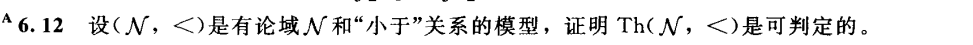
\includegraphics[width=\textwidth]{chapters/imgs/hw_6_12.png}
  \caption{}
  \label{fig:hw_6_12}
\end{figure}

\begin{answerred}
\paragraph{解答.}
我们把语言
\[
\{<\}
\]
中的每个公式有效翻译成语言
\[
\{+\}
\]
中的公式。关键观察是：在自然数上，
\[
x<y
\iff
\exists z\,\bigl(z\ne 0 \wedge x+z=y\bigr).
\]

\medskip
因此，对任意一阶句子 $\varphi$（其唯一非逻辑符号是 $<$），都可以机械地构造一个新句子 $\varphi^\sharp$（其唯一非逻辑符号是 $+$），方法是把 $\varphi$ 中每个原子式
\[
x<y
\]
都替换成
\[
\exists z\,\bigl(z\ne 0 \wedge x+z=y\bigr),
\]
其余逻辑联结词和量词保持不变。

\medskip
这样构造满足：
\[
(\mathbb N,<)\models \varphi
\iff
(\mathbb N,+)\models \varphi^\sharp.
\]
原因很直接：在自然数结构上，
\[
<
\]
与
\[
\exists z\,(z\ne 0\wedge x+z=y)
\]
定义的是同一个关系，所以替换前后真值不变。

\medskip
现在利用已知结果：
\[
\mathrm{Th}(\mathbb N,+)
\]
是可判定的。于是要判定任意句子
\[
\varphi\in \mathrm{Th}(\mathbb N,<),
\]
只需：

\begin{enumerate}[label=(\arabic*), leftmargin=2.5em]
  \item 有效地把 $\varphi$ 翻译成 $\varphi^\sharp$；
  \item 用
  \[
  \mathrm{Th}(\mathbb N,+)
  \]
  的判定算法判定 $\varphi^\sharp$ 是否为真。
\end{enumerate}

若 $\varphi^\sharp$ 在
\[
(\mathbb N,+)
\]
中为真，则 $\varphi$ 在
\[
(\mathbb N,<)
\]
中为真；反之亦然。故
\[
\mathrm{Th}(\mathbb N,<)
\]
可判定。$\blacksquare$

\begin{answernote}
\paragraph{解释.}
这里的符号 $\models$ 表示“满足”关系：$\mathcal M\models\psi$ 的意思是句子 $\psi$ 在结构 $\mathcal M$ 中为真。因此
\[
(\mathbb N,<)\models \varphi
\iff
(\mathbb N,+)\models \varphi^\sharp
\]
就是说，原句子 $\varphi$ 在自然数的小于结构中为真，当且仅当翻译后的句子 $\varphi^\sharp$ 在自然数的加法结构中为真。

\medskip
需要注意的是，这里的存在量词不是说判定器要盲目枚举
\[
z=1,2,3,\ldots
\]
直到找到为止。若 $x,y$ 已经被赋为具体自然数，那么
\[
x+z=y
\]
一旦成立就必有 $z\le y$，所以只需要检查有限多个候选 $z=1,\ldots,y$。特别地，当 $x>y$ 时，对任意 $z\in\mathbb N$ 都有
\[
x+z\ge x>y,
\]
因此根本不存在满足 $x+z=y$ 的 $z$。

\medskip
对一般的一阶句子，证明也不是靠对量词取值作无界搜索，而是先把句子有效翻译到只含加法的语言中，再调用已知的
\[
\mathrm{Th}(\mathbb N,+)
\]
的判定算法。也就是说，有限步停机性来自 Presburger 算术的可判定性，而不是来自对存在量词的朴素枚举。

\medskip
这里的核心不是重新发明一个关于 $<$ 的判定器，而是把“小于”翻译成“加法存在一个正增量”。一旦这个翻译是有效的，而
\[
(\mathbb N,+)
\]
的理论已经可判定，那么
\[
(\mathbb N,<)
\]
的理论也就跟着可判定。

\end{answernote}
\end{answerred}
\subsection*{6.14}

\begin{figure}[H]
  \centering
  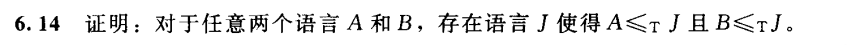
\includegraphics[width=\textwidth]{chapters/imgs/hw_6_14.png}
  \caption{}
  \label{fig:hw_6_14}
\end{figure}

\begin{answerred}
\paragraph{解答.}
定义语言
\[
J=\{0x\mid x\in A\}\cup \{1x\mid x\in B\}.
\]
我们证明
\[
A\le_T J
\qquad\text{且}\qquad
B\le_T J.
\]

\paragraph{证明 \(A\le_T J\).}
构造带预言机 $J$ 的图灵机 $M_A^J$：在输入 $x$ 上，仅向预言机询问一次
\[
0x\in J\;?
\]
若预言机回答“是”，则接受；否则拒绝。

由 $J$ 的定义，
\[
0x\in J
\iff
x\in A.
\]
因此 $M_A^J$ 判定 $A$，从而
\[
A\le_T J.
\]

\paragraph{证明 \(B\le_T J\).}
同理，构造带预言机 $J$ 的图灵机 $M_B^J$：在输入 $x$ 上询问
\[
1x\in J\;?
\]
并按照答案接受或拒绝。因为
\[
1x\in J
\iff
x\in B,
\]
所以 $M_B^J$ 判定 $B$，从而
\[
B\le_T J.
\]

\medskip
于是我们找到了一个语言 $J$，使得
\[
A\le_T J
\qquad\text{且}\qquad
B\le_T J.
\]
命题得证。$\blacksquare$

\begin{answernote}
\paragraph{解释.}
这个构造就是把两个语言“并排打包”进一个新语言里。前缀 $0$ 表示“这是关于 $A$ 的问题”，前缀 $1$ 表示“这是关于 $B$ 的问题”。于是同一个预言机 $J$ 同时包含了两边的信息。

\end{answernote}
\end{answerred}
\subsection*{6.17}

\begin{figure}[H]
  \centering
  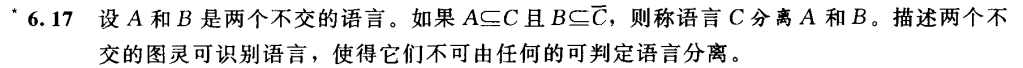
\includegraphics[width=\textwidth]{chapters/imgs/hw_6_17.png}
  \caption{}
  \label{fig:hw_6_17}
\end{figure}

\begin{answerred}
\paragraph{解答.}
取
\[
A=\{\langle M\rangle\mid M \text{ 接受 } \langle M\rangle\},
\]
\[
B=\{\langle M\rangle\mid M \text{ 拒绝 } \langle M\rangle\}.
\]

\paragraph{1. \(A\) 与 \(B\) 不相交且都是图灵可识别的.}
显然
\[
A\cap B=\varnothing,
\]
因为一台图灵机在同一个输入上不可能既接受又拒绝。

对 $A$，给定输入 $\langle M\rangle$，直接模拟 $M$ 在输入 $\langle M\rangle$ 上的运行；若 $M$ 接受，则接受。故 $A$ 是图灵可识别的。

对 $B$，给定输入 $\langle M\rangle$，同样模拟 $M$ 在输入 $\langle M\rangle$ 上的运行；若 $M$ 拒绝，则接受。故 $B$ 也是图灵可识别的。

\paragraph{2. 证明它们不能被任何可判定语言分离.}
反设存在一个可判定语言 $C$，满足
\[
A\subseteq C
\qquad\text{且}\qquad
B\subseteq \overline C.
\]
设图灵机 $R$ 判定 $C$。构造图灵机 $D$：

\begin{myalgo}{由分离器 $R$ 构造的图灵机 $D$}
\begin{algorithmic}[1]
  \Require 输入 $x$
  \Ensure 在 $R$ 的答案上对角化
  \State 在输入 $x$ 上运行 $R$
  \If{$R$ 接受}
    \State \textbf{拒绝}
  \Else
    \State \textbf{接受}
  \EndIf
\end{algorithmic}
\end{myalgo}

现在考虑 $\langle D\rangle$。

\medskip
若
\[
\langle D\rangle\in C,
\]
则 $R$ 在输入 $\langle D\rangle$ 上接受，因此 $D$ 在输入 $\langle D\rangle$ 上拒绝。于是
\[
\langle D\rangle\in B.
\]
但
\[
B\subseteq \overline C,
\]
故
\[
\langle D\rangle\notin C,
\]
矛盾。

\medskip
若
\[
\langle D\rangle\notin C,
\]
则 $R$ 在输入 $\langle D\rangle$ 上拒绝，因此 $D$ 在输入 $\langle D\rangle$ 上接受。于是
\[
\langle D\rangle\in A.
\]
但
\[
A\subseteq C,
\]
故
\[
\langle D\rangle\in C,
\]
仍然矛盾。

\medskip
因此不存在任何可判定语言 $C$ 能把 $A$ 与 $B$ 分离开。故题目所求的两个语言就是上述 $A$ 与 $B$。$\blacksquare$

\begin{answernote}
\paragraph{解释.}
这两个语言分别记录“机器在自己描述上接受”和“机器在自己描述上拒绝”。如果某个可判定语言真能把这两种情况完全分开，就能像标准对角化那样造出一台在自己描述上永远与这个分离器作对的机器，于是立刻矛盾。

\end{answernote}
\end{answerred}
\subsection*{6.22}

\begin{figure}[H]
  \centering
  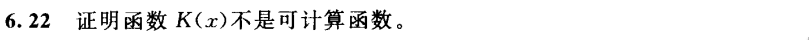
\includegraphics[width=\textwidth]{chapters/imgs/hw_6_22.png}
  \caption{}
  \label{fig:hw_6_22}
\end{figure}

\begin{answerred}
\paragraph{解答.}
反设函数
\[
K(x)
\]
是可计算的。我们将导出矛盾。

\medskip
在这个假设下，构造如下图灵机 $M$：给定输入 $n$（用二进制编码），$M$ 依次枚举所有字符串
\[
x
\]
并计算
\[
K(x),
\]
直到找到字典序最小的满足
\[
K(x)>n
\]
的字符串，然后输出该字符串。

\begin{myalgo}{假设 $K$ 可计算时构造的机器 $M$}
\begin{algorithmic}[1]
  \Require 输入正整数 $n$
  \Ensure 输出字典序最小的满足 $K(x)>n$ 的字符串
  \ForAll{字符串 $x$，按字典序枚举}
    \State 计算 $K(x)$
    \If{$K(x)>n$}
      \State 输出 $x$ 并停机
    \EndIf
  \EndFor
\end{algorithmic}
\end{myalgo}

先说明这样的字符串一定存在。因为长度至多为 $n$ 的描述只有有限多个，所以满足
\[
K(x)\le n
\]
的字符串也只有有限多个；而字符串总数是无限的，因此必然存在某个 $x$ 使得
\[
K(x)>n.
\]
故机器 $M$ 对每个输入 $n$ 都会停机。

\medskip
设机器 $M$ 在输入 $n$ 时输出的字符串为 $x_n$。由构造，
\[
K(x_n)>n.
\]

另一方面，$x_n$ 可以由“机器 $M$ 的固定描述”加上“输入 $n$ 的编码”唯一确定。因此存在常数 $c$，使得对所有 $n$，
\[
K(x_n)\le |\langle n\rangle|+c.
\]
由于 $n$ 采用二进制编码，
\[
|\langle n\rangle|\le \lceil \log_2 n\rceil + O(1),
\]
所以存在常数 $c'$，使得
\[
K(x_n)\le \log_2 n + c'.
\]

\medskip
综上，对充分大的 $n$，
\[
n < K(x_n)\le \log_2 n + c',
\]
这是不可能的，因为
\[
\log_2 n + c' < n
\]
当 $n$ 足够大时成立。

\medskip
矛盾说明最初假设错误。因此函数
\[
K(x)
\]
不是可计算函数。$\blacksquare$

\begin{answernote}
\paragraph{解释.}
这里的 $K(x)$ 是字符串 $x$ 的描述复杂度，也就是 Kolmogorov 复杂度。教材在第 6.4 节的 Definition 6.23 中先定义 $d(x)$ 为 $x$ 的最短描述：它是最短的串 $\langle M,w\rangle$，其中图灵机 $M$ 在输入 $w$ 上停机并输出 $x$；若有多个同样短的描述，就取字典序最小的那个。然后定义
\[
K(x)=|d(x)|.
\]
所以 $K(x)$ 衡量的是生成 $x$ 所需的最短有效描述长度。

\medskip
证明中
\[
K(x_n)\le |\langle n\rangle|+c
\]
的原因是：$x_n$ 是固定机器 $M$ 在输入 $n$ 上输出的字符串。因此，只要给出“机器 $M$ 的固定描述”以及“输入 $n$ 的编码”，就能重新运行 $M(n)$ 并唯一得到 $x_n$。所以
\[
\langle M,n\rangle
\]
本身就是 $x_n$ 的一个合法描述。由于 $K(x_n)$ 取的是最短描述长度，它不会比这个具体描述更长。

其中 $M$ 已经固定，$\langle M\rangle$ 的长度以及配对编码的额外开销都可以并入一个常数 $c$，于是只剩下输入 $n$ 的编码长度：
\[
K(x_n)\le |\langle n\rangle|+c.
\]
又因为 $n$ 采用二进制编码，所以
\[
|\langle n\rangle|\le \lceil \log_2 n\rceil+O(1),
\]
从而可把常数项合并，得到
\[
K(x_n)\le \log_2 n+c'.
\]
这正是教材 Theorem 6.24 后面的思想：为了给 $K(x)$ 找上界，只需要展示一个能生成 $x$ 的描述；最短描述只会更短。

\medskip
这是 Kolmogorov 复杂度版本的 Berry 悖论。若 $K$ 真能计算，我们就能有效地找到“第一个复杂度大于 $n$ 的串”。但这样一个串又被“这台寻找它的机器 + 参数 $n$”简短地描述了，于是它反而不该那么复杂。
\end{answernote}
\end{answerred}

\subsection*{本章总结}

这一章的题目集中在可计算性理论的几个高级工具上：预言机与图灵归约、递归定理式的自引用、逻辑理论的可判定性、以及 Kolmogorov 复杂度。它们表面上分散，但共同主题是：当普通判定器不够用时，我们怎样比较问题的计算能力，或者证明某些能力边界仍然无法突破。

\subsubsection*{预言机与图灵归约}

图灵归约
\[
A\le_T B
\]
表示“若可以把 $B$ 当作预言机使用，就能判定 $A$”。6.3 的传递性说明：如果 $A$ 的判定过程只需要询问 $B$，而每个 $B$ 的询问又能借助 $C$ 回答，那么这些询问可以逐层替换，最终得到一个只使用 $C$ 的判定器。这就是预言机计算中的组合原则。

6.14 的构造
\[
J=\{0x\mid x\in A\}\cup\{1x\mid x\in B\}
\]
则说明：两个语言可以被打包进同一个预言机语言中。前缀 $0$ 和 $1$ 分别标记问题来自 $A$ 还是 $B$，因此 $J$ 同时携带了两边的信息。

\subsubsection*{相对化与对角化}

6.4 的重点是：即使机器已经拥有
\[
A_{\mathrm{TM}}
\]
作为预言机，仍然不能判定“带这个预言机的机器是否接受输入”的更高一层问题
\[
A_{\mathrm{TM}}^{A_{\mathrm{TM}}}.
\]
证明仍然使用对角化。

这里的“对角化”不是线性代数中的对角化，而是计算理论中的自指取反技巧。可以把所有机器 $M_i$ 和所有输入 $\langle M_j\rangle$ 排成一张表，对角线位置是
\[
M_i(\langle M_i\rangle),
\]
也就是“机器在自己的描述上运行”。对角化构造一台新机器 $D$，专门在这些对角线位置上与假想判定器的预测相反：若判定器说接受，$D$ 就拒绝；若判定器说不接受，$D$ 就接受。最后把 $D$ 自己放到自己的输入上，就会得到
\[
D \text{ 接受 } \langle D\rangle
\iff
D \text{ 不接受 } \langle D\rangle
\]
这种矛盾。

6.17 中的不可分离证明也是同一个思想。若存在可判定语言 $C$ 能把
\[
A=\{\langle M\rangle\mid M \text{ 接受 } \langle M\rangle\}
\]
和
\[
B=\{\langle M\rangle\mid M \text{ 拒绝 } \langle M\rangle\}
\]
完全分开，就可以构造一台机器 $D$ 在自己的描述上永远与这个分离器的答案相反，从而推出矛盾。因此，对角化的核心不是某个特殊语言，而是“假设有一个全局正确的判定器，再构造一个专门反着它来的自指对象”。

\subsubsection*{递归定理与自引用}

6.7 展示了递归定理背后的不动点思想：对一个可计算变换 $t$，可以寻找某种意义上不被 $t$ 改变行为的机器。这里的例子是把接受态和拒绝态交换。如果机器在所有输入上都一直循环，那么接受态和拒绝态根本不会被访问，交换它们不改变识别的语言。因此它给出了一个直观的不动点。

这和对角化一样都涉及“机器谈论自己”，但方向不同：对角化用自引用制造矛盾，递归定理则说明图灵机可以在严格意义上获得并利用自己的描述。

\subsubsection*{逻辑理论与可判定性}

6.10 和 6.12 属于逻辑理论部分。6.10 是模型构造题：把一个关系符号解释成等号，就得到满足自反、对称、传递的结构，也就是一个等价关系模型。

6.12 的关键是把自然数上的小于关系定义进加法结构：
\[
x<y
\iff
\exists z\,(z\ne 0\wedge x+z=y).
\]
因此，任何只含 $<$ 的句子都可以有效翻译成只含 $+$ 的句子。由于
\[
\mathrm{Th}(\mathbb N,+)
\]
即 Presburger 算术是可判定的，翻译之后就能调用它的判定算法，从而得到
\[
\mathrm{Th}(\mathbb N,<)
\]
也是可判定的。这里要注意，存在量词本身不是要求无界枚举；有限步停机性来自加法理论的判定算法。

\subsubsection*{Kolmogorov 复杂度}

6.22 讨论描述复杂度
\[
K(x),
\]
也就是生成字符串 $x$ 所需的最短有效描述长度。证明 $K$ 不可计算的思路是 Berry 悖论式的：如果 $K$ 可计算，就能构造机器找出“第一个复杂度大于 $n$ 的字符串”。但这个字符串又可以被“这台机器加参数 $n$”很短地描述出来，于是它不可能真的有那么高的复杂度，矛盾。

这一部分说明，计算不可判定性不仅出现在“机器是否接受输入”这类问题中，也会出现在“一个对象到底含有多少可压缩信息”这种信息论式问题中。

\subsubsection*{整体脉络}

本章可以看成三条主线的交汇：
\begin{enumerate}[label=(\arabic*), leftmargin=2.5em]
  \item 用预言机和图灵归约比较问题之间的相对计算能力；
  \item 用对角化、递归定理和不可分离性刻画自引用带来的不可判定边界；
  \item 用逻辑理论和 Kolmogorov 复杂度展示可计算性思想在数理逻辑与信息描述中的应用。
\end{enumerate}

这些题共同强调一点：给计算模型增加工具并不等于消除所有不可判定性。预言机能提升能力，但仍会出现更高层的问题；逻辑语言可以互相翻译，但可判定性依赖于目标理论本身；字符串可以有描述复杂度，但这个复杂度函数本身不可计算。

\clearpage
